% Adjust these for the path of the theme and its graphics, relative to this file
%\usepackage{beamerthemeFalmouthGamesAcademy}
\usepackage{../../beamerthemeFalmouthGamesAcademy}
\usepackage{multimedia}
\graphicspath{ {../../} }

% Default language for code listings
\lstset{language=Python}

% For strikethrough effect
\usepackage[normalem]{ulem}
\usepackage{wasysym}

\usepackage{pdfpages}

% http://www.texample.net/tikz/examples/state-machine/
\usetikzlibrary{arrows,automata,tikzmark,calc}

\usepackage{algpseudocode}
\usepackage{qtree}

\newcommand{\modulecode}{COMP260}\newcommand{\moduletitle}{Distributed Systems}\newcommand{\sessionnumber}{5}

\begin{document}
\title{\sessionnumber: Data Structures II}
\subtitle{\modulecode: \moduletitle}

\frame{\titlepage} 

\begin{frame}
	\frametitle{Learning outcomes}
	\begin{itemize}
		\item \textbf{Define} the key concepts of graph theory
		\item \textbf{Distinguish} advanced data structures such as trees, DAGs and graphs
		\item \textbf{Determine} the complexity of accessing and manipulating data in these data structures
		\item \textbf{Choose} the correct data structure for a given task
	\end{itemize}
\end{frame}

\part{More data structures}
\frame{\partpage}

\begin{frame}{Stacks and queues}
	\begin{columns}
		\pause
		\begin{column}{0.3\textwidth}
			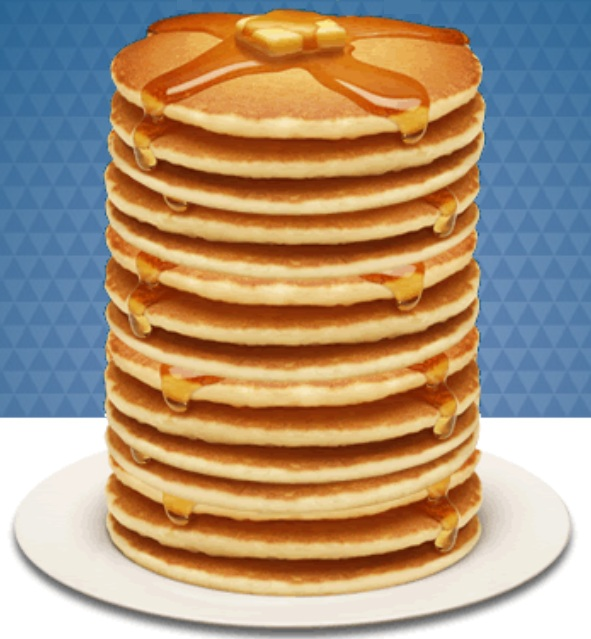
\includegraphics[width=\textwidth]{stack}
		\end{column}
		\begin{column}{0.68\textwidth}
			\begin{itemize}
				\item A \textbf{stack} is a \textbf{last-in first-out (LIFO)} data structure
				\pause\item Items can be \textbf{pushed} to the \textbf{top} of the stack
				\pause\item Items can be \textbf{popped} from the \textbf{top} of the stack
			\end{itemize}
		\end{column}
	\end{columns}
	\begin{columns}
		\pause
		\begin{column}{0.3\textwidth}
			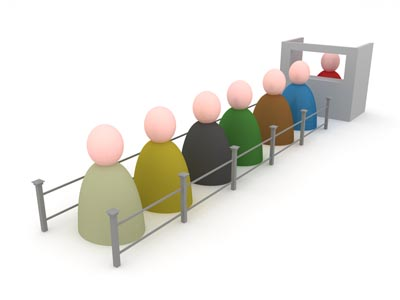
\includegraphics[width=\textwidth]{queue}
		\end{column}
		\begin{column}{0.68\textwidth}
			\begin{itemize}
				\item A \textbf{queue} is a \textbf{first-in first-out (LIFO)} data structure
				\pause\item Items can be \textbf{enqueued} to the \textbf{back} of the queue
				\pause\item Items can be \textbf{dequeued} from the \textbf{front} of the queue
			\end{itemize}
		\end{column}
	\end{columns}
\end{frame}

\begin{frame}{Stacks and queues in Python}
	\begin{itemize}
		\pause\item Stacks can be implemented efficiently as lists
		\pause\item Queues can be implemented as lists, but not efficiently
		\pause\item \lstinline{deque} (from the \lstinline{collections} module) implements an efficient
			\textbf{double-ended queue}
		\pause\item Inserting and removing elements from the start and end of a \lstinline{deque} is $O(1)$
	\end{itemize}
\end{frame}

\begin{frame}{Graphs}
	\begin{columns}
		\pause
		\begin{column}{0.3\textwidth}
			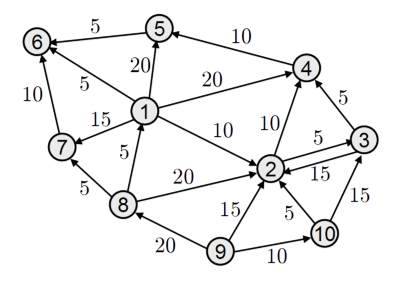
\includegraphics[width=\textwidth]{graph1}
			\par
			\vspace{2ex}
			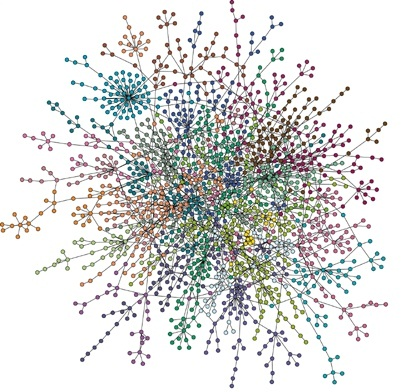
\includegraphics[width=\textwidth]{graph2}
		\end{column}
		\begin{column}{0.68\textwidth}
			\begin{itemize}
				\pause\item A \textbf{graph} is defined by:
					\begin{itemize}
						\pause\item A collection of \textbf{nodes} or \textbf{vertices} (points)
						\pause\item A collection of \textbf{edges} or \textbf{arcs} (undirected lines or directed arrows between points)
					\end{itemize}
				\pause\item Often used to model \textbf{networks} (e.g.\ social networks, transport networks, game levels, finite state automata, ...)
			\end{itemize}
		\end{column}
	\end{columns}
\end{frame}

\begin{frame}{Trees}
	\begin{columns}
		\pause
		\begin{column}{0.3\textwidth}
			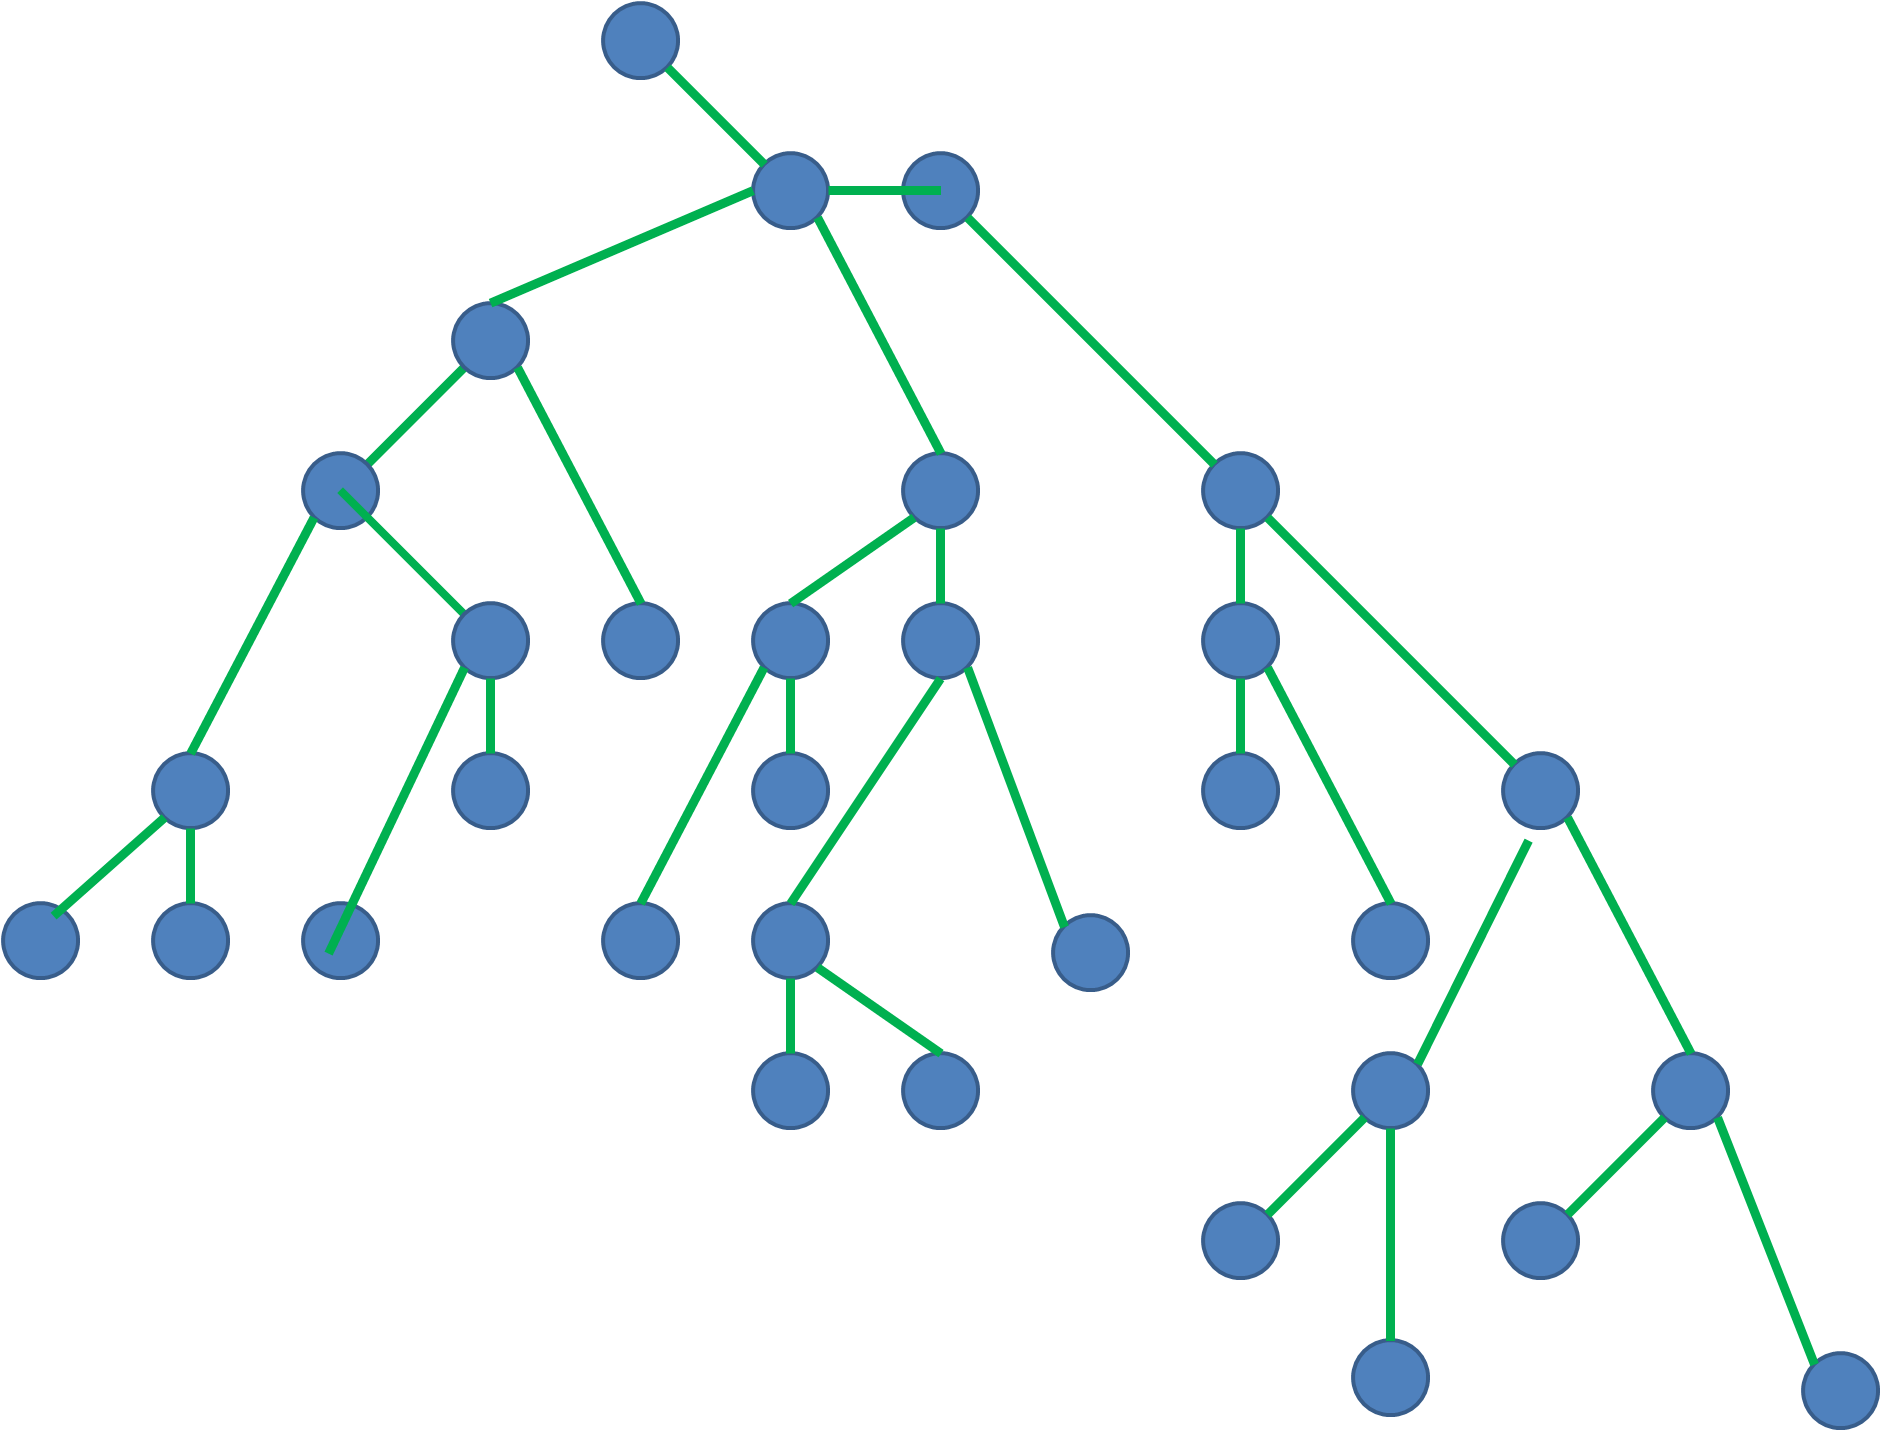
\includegraphics[width=\textwidth]{tree2}
			\par
			\vspace{2ex}
			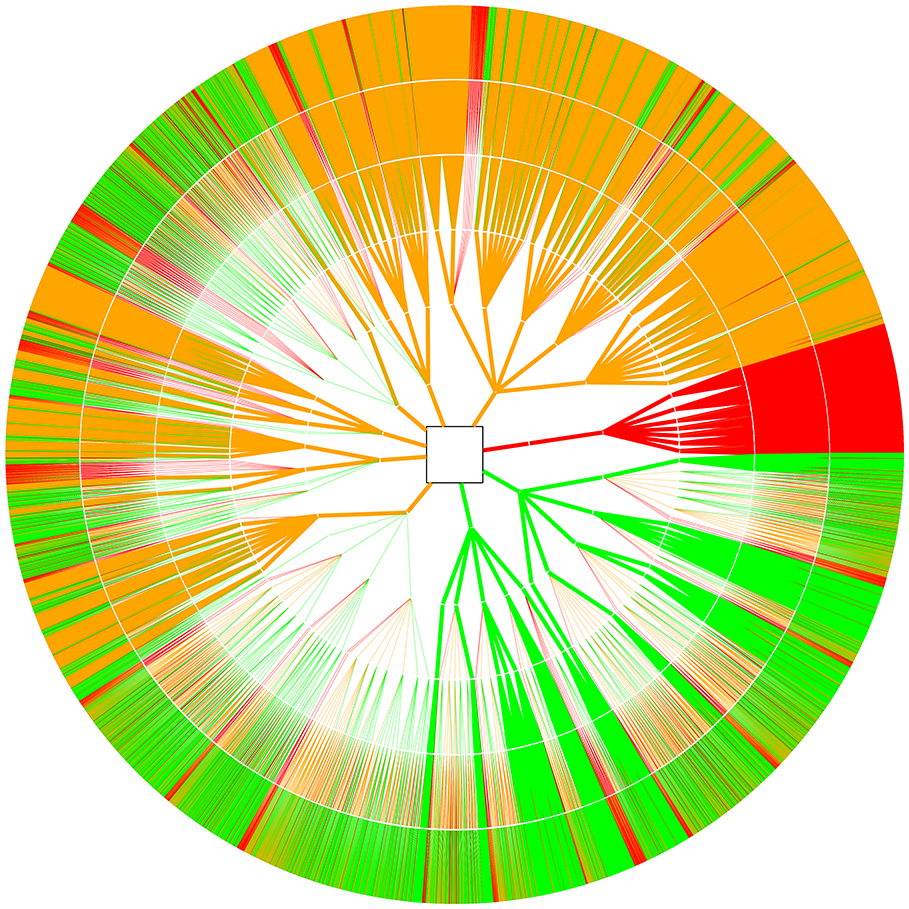
\includegraphics[width=\textwidth]{tree}
		\end{column}
		\begin{column}{0.68\textwidth}
			\begin{itemize}
				\pause\item A \textbf{tree} is a special type of directed graph where:
					\begin{itemize}
						\pause\item One node (the \textbf{root}) has no incoming edges
						\pause\item All other nodes have exactly 1 incoming edge
					\end{itemize}
				\pause\item Edges go from \textbf{parent} to \textbf{child}
					\begin{itemize}
						\pause\item All nodes except the root have exactly one parent
						\pause\item Nodes can have 0, 1 or many children
					\end{itemize}
				\pause\item Used to model \textbf{hierarchies} (e.g.\ file systems, object inheritance, scene graphs, state-action trees, ...)
			\end{itemize}
		\end{column}
	\end{columns}
\end{frame}


\part{Linked lists}
\frame{\partpage}

\begin{frame}{Linked list}
	\begin{itemize}
		\pause\item Composed of a number of \textbf{nodes}
		\pause\item Each node contains:
			\begin{itemize}
		 		\pause\item An \textbf{item} --- the actual data to be stored
		 		\pause\item A pointer or reference to the \textbf{previous node} in the list (null for the first item)
		 		\pause\item A pointer or reference to the \textbf{next node} in the list (null for the last item)
			\end{itemize}
	\end{itemize}
	\pause
	\vspace{2ex}
	\begin{center}
	    \setlength{\tabcolsep}{0.2em}
		\begin{tabular}{|c|c|c|}
			\hline
			{\tiny prev} & {\tiny item} & {\tiny next} \\
			$\times$ & \texttt{\footnotesize first} & \tikzmark{nexta} \\\hline
		\end{tabular}
		\qquad
		\begin{tabular}{|c|c|c|}
			\hline
			{\tiny prev} & {\tiny item} & {\tiny next} \\
			\tikzmark{prevb} & \texttt{\footnotesize second} & \tikzmark{nextb} \\\hline
		\end{tabular}
		\qquad
		\begin{tabular}{|c|c|c|}
			\hline
			{\tiny prev} & {\tiny item} & {\tiny next} \\
			\tikzmark{prevc} & \texttt{\footnotesize third} & $\times$ \\\hline
		\end{tabular}
		
\begin{tikzpicture}
			[
			  remember picture,
			  overlay,
			  -latex,
			  yshift=0.5ex,
			  shorten >=1pt,
			  shorten <=1pt,
			]
			\draw ($ ({pic cs:nexta}) + (0, 0.5ex) $) to ($ ({pic cs:prevb}) + (-1.2ex, 0.5ex) $);
			\draw ($ ({pic cs:nextb}) + (0, 0.5ex) $) to ($ ({pic cs:prevc}) + (-1.2ex, 0.5ex) $);
			\draw ($ ({pic cs:prevb}) + (0, -0.5ex) $) to ($ ({pic cs:nexta}) + (1.2ex, -0.5ex) $);
			\draw ($ ({pic cs:prevc}) + (0, -0.5ex) $) to ($ ({pic cs:nextb}) + (1.2ex, -0.5ex) $);
		\end{tikzpicture}
	\end{center}
\end{frame}

\newcommand{\footnoteref}[1]{$^{\text{\ref{#1}}}$}

\begin{frame}{Linked lists vs arrays}
	\begin{center}
		\begin{tabular}{|r|l|l|}
			\hline
			\textbf{Operation} & \textbf{Array} & \textbf{Linked list} \\\hline
			\pause Append & $O(1)$ & $O(1)$ \footnote{\label{f:llend}If we already have a reference to the last node} \\
			\pause Pop & $O(1)$ & $O(1)$ \footnoteref{f:llend} \\
			\pause Index lookup & $O(1)$ & $O(n)$ \\
			\pause Count elements & $O(1)$ & $O(n)$ \\
			\pause Insert & $O(n)$ & $O(1)$ \footnote{\label{f:llinsert}If we already have a reference to the relevant node} \\
			\pause Delete & $O(n)$ & $O(1)$ \footnoteref{f:llinsert} \\
			\hline
		\end{tabular}
	\end{center}
\end{frame}

\begin{frame}{Implementing a linked list}
\end{frame}

\part{Graphs and trees}
\frame{\partpage}

\begin{frame}{Graphs}
	\begin{columns}
		\pause
		\begin{column}{0.3\textwidth}
			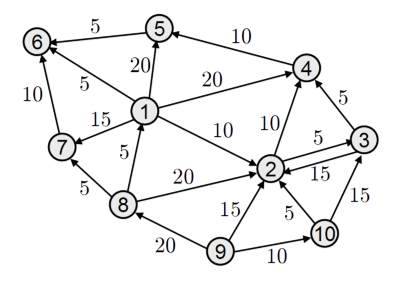
\includegraphics[width=\textwidth]{graph1}
			\par
			\vspace{2ex}
			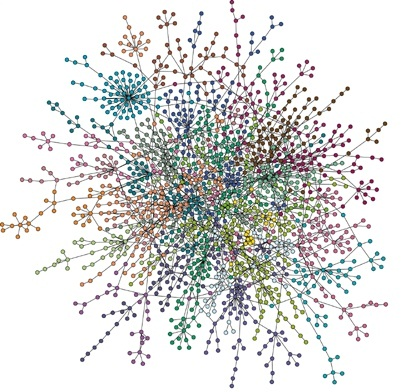
\includegraphics[width=\textwidth]{graph2}
		\end{column}
		\begin{column}{0.68\textwidth}
			\begin{itemize}
				\pause\item A \textbf{graph} is defined by:
					\begin{itemize}
						\pause\item A collection of \textbf{nodes} or \textbf{vertices} (points)
						\pause\item A collection of \textbf{edges} or \textbf{arcs} (lines or arrows between points)
					\end{itemize}
				\pause\item Often used to model \textbf{networks} (e.g.\ social networks, transport networks, game levels, automata, ...)
				\pause\item \textbf{Directed} graph: edges are arrows
				\pause\item \textbf{Undirected} graph: edges are lines
			\end{itemize}
		\end{column}
	\end{columns}
\end{frame}

\begin{frame}{Drawing graphs}
    \begin{itemize}
        \pause\item A graph does not necessarily specify the physical \textbf{positions} of its nodes
        \pause\item E.g.\ these are technically the same graph:
    \end{itemize}
    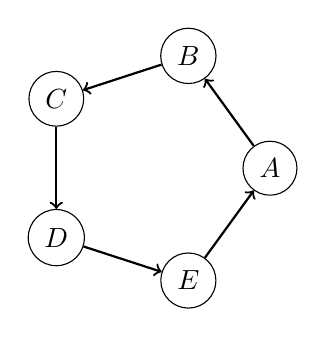
\begin{tikzpicture}
        \node[draw, circle] (a) at (0:1.5) {$A$};
        \node[draw, circle] (b) at (72:1.5) {$B$};
        \node[draw, circle] (c) at (144:1.5) {$C$};
        \node[draw, circle] (d) at (216:1.5) {$D$};
        \node[draw, circle] (e) at (288:1.5) {$E$};
        \draw[thick,->] (a) -- (b);
        \draw[thick,->] (b) -- (c);
        \draw[thick,->] (c) -- (d);
        \draw[thick,->] (d) -- (e);
        \draw[thick,->] (e) -- (a);
    \end{tikzpicture}
    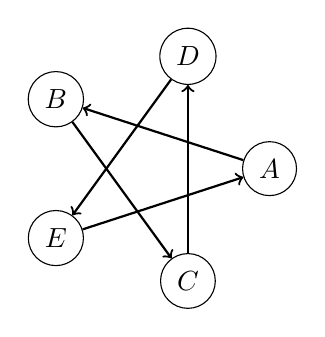
\begin{tikzpicture}
        \node[draw, circle] (a) at (0:1.5) {$A$};
        \node[draw, circle] (b) at (144:1.5) {$B$};
        \node[draw, circle] (c) at (288:1.5) {$C$};
        \node[draw, circle] (d) at (72:1.5) {$D$};
        \node[draw, circle] (e) at (216:1.5) {$E$};
        \draw[thick,->] (a) -- (b);
        \draw[thick,->] (b) -- (c);
        \draw[thick,->] (c) -- (d);
        \draw[thick,->] (d) -- (e);
        \draw[thick,->] (e) -- (a);
    \end{tikzpicture}
    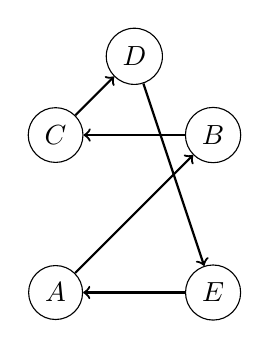
\begin{tikzpicture}
        \node[draw, circle] (a) at (0,0) {$A$};
        \node[draw, circle] (b) at (2,2) {$B$};
        \node[draw, circle] (c) at (0,2) {$C$};
        \node[draw, circle] (d) at (1,3) {$D$};
        \node[draw, circle] (e) at (2,0) {$E$};
        \draw[thick,->] (a) -- (b);
        \draw[thick,->] (b) -- (c);
        \draw[thick,->] (c) -- (d);
        \draw[thick,->] (d) -- (e);
        \draw[thick,->] (e) -- (a);
    \end{tikzpicture}
\end{frame}

\begin{frame}{Trees}
	\begin{columns}
		\pause
		\begin{column}{0.3\textwidth}
			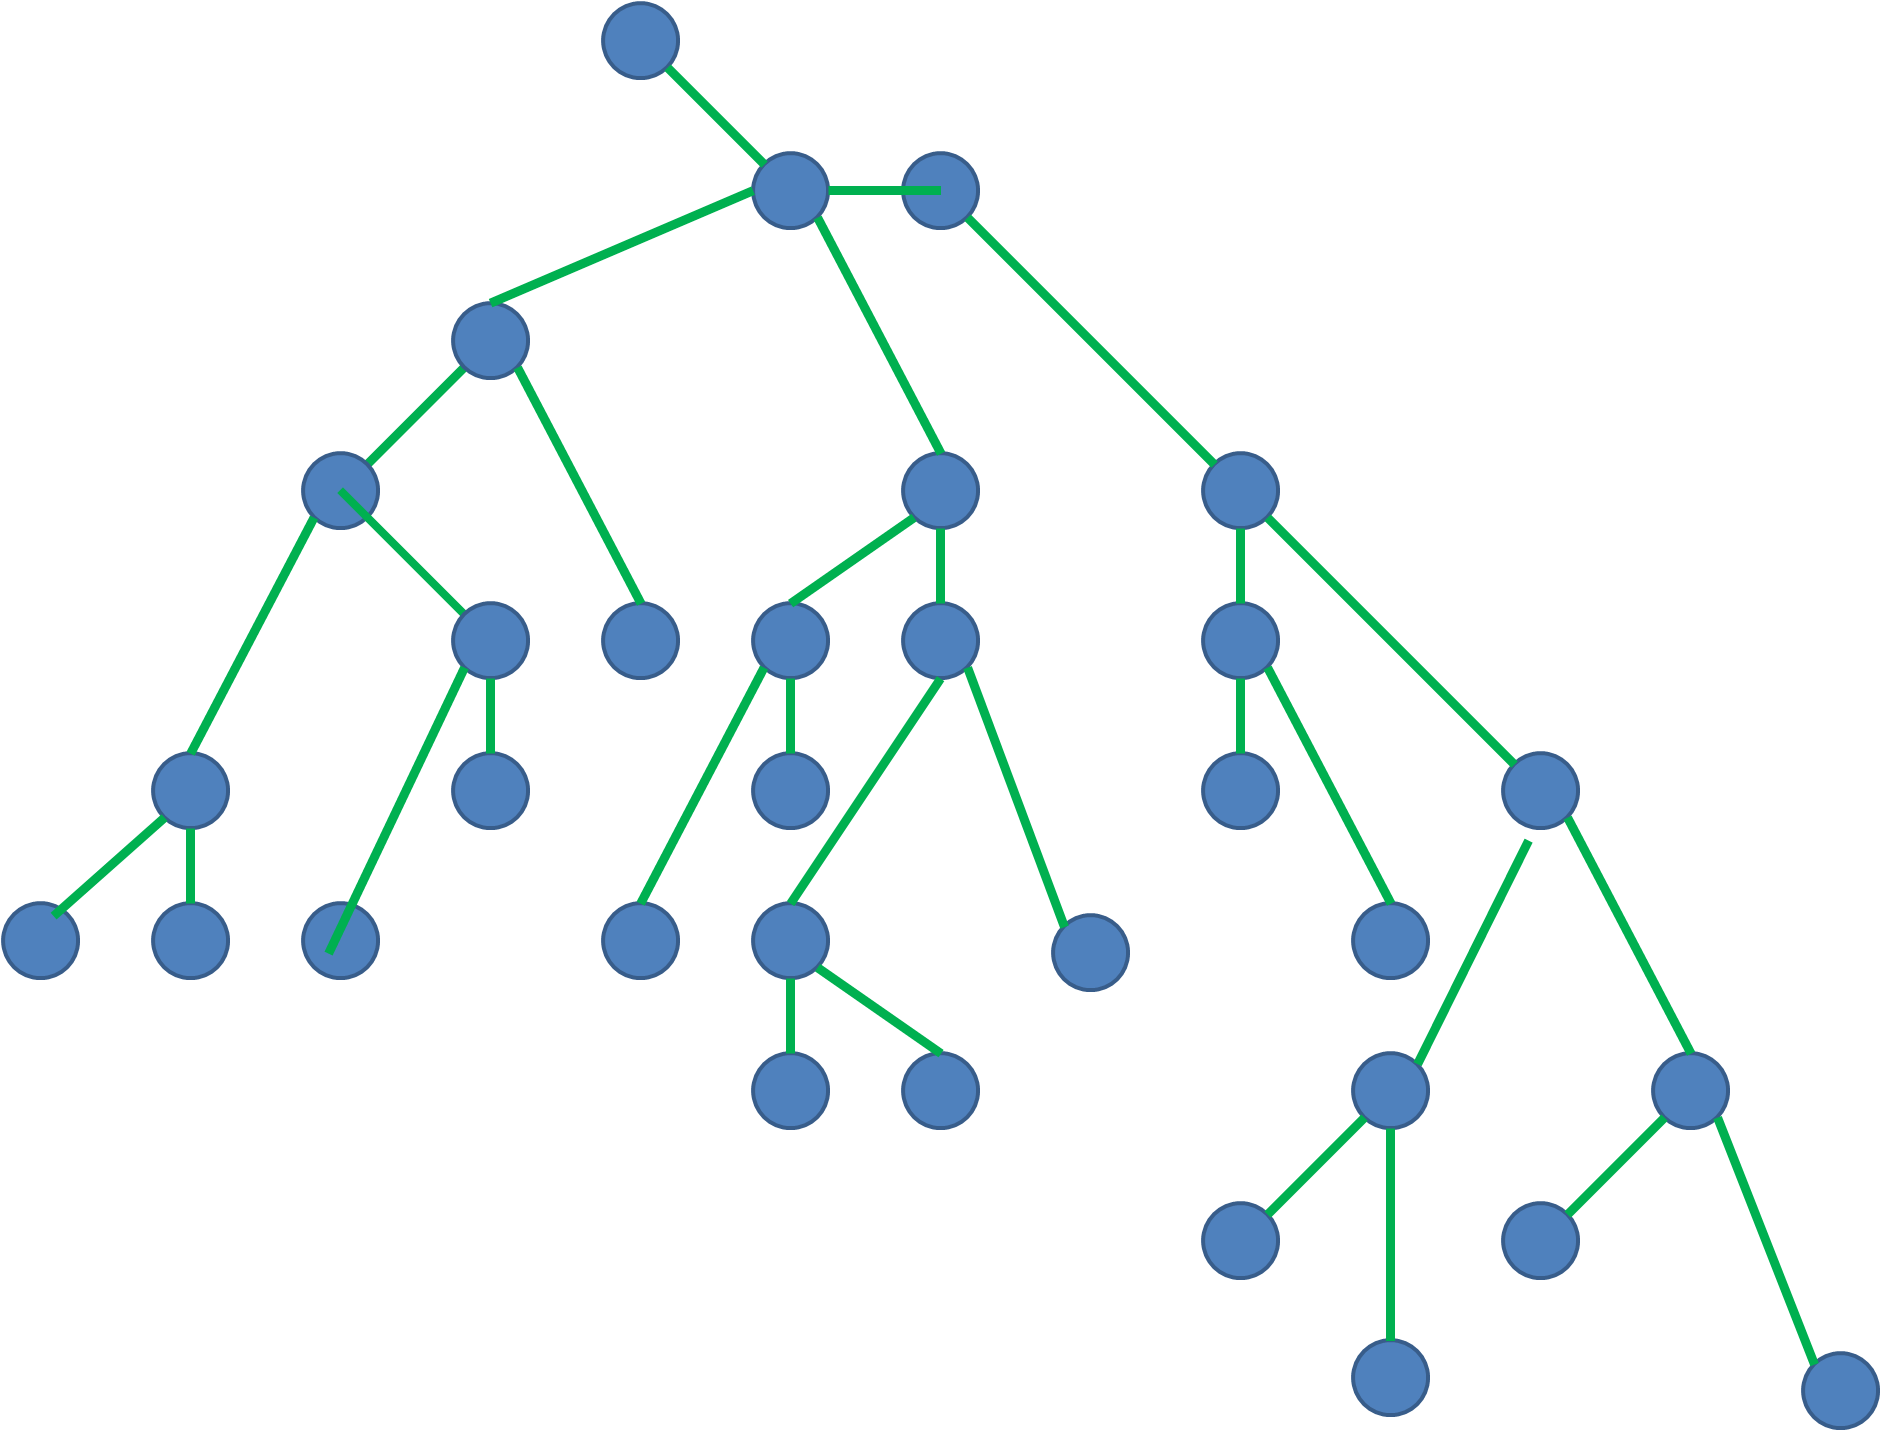
\includegraphics[width=\textwidth]{tree2}
			\par
			\vspace{2ex}
			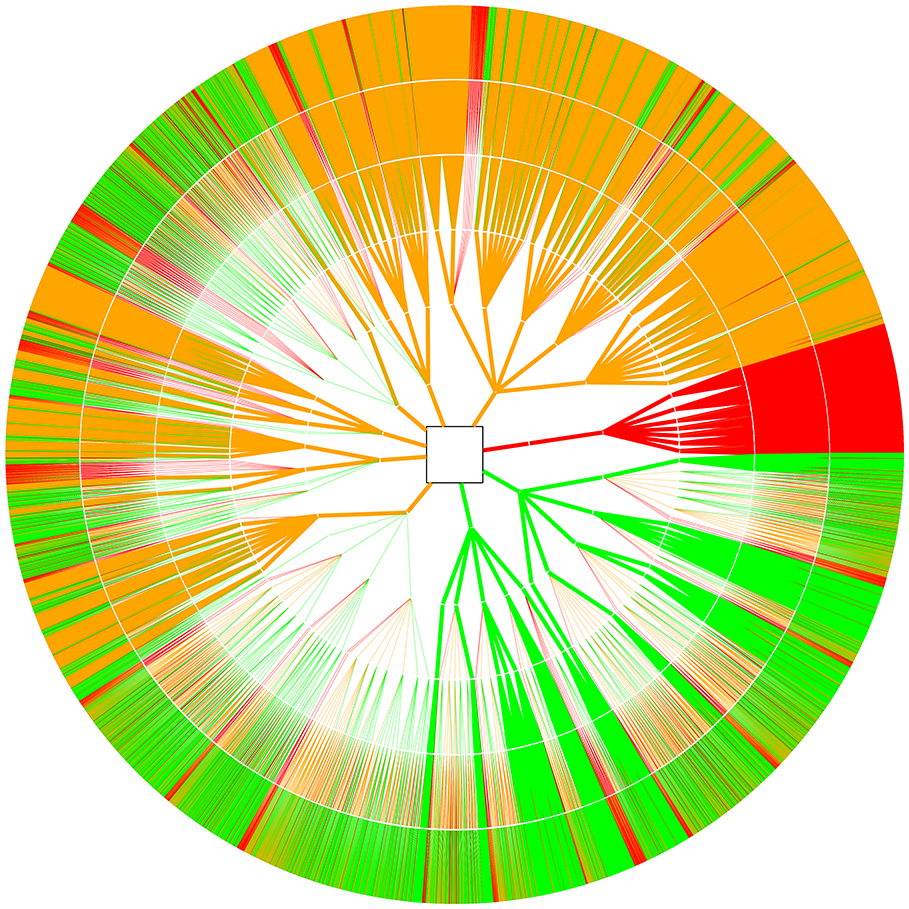
\includegraphics[width=\textwidth]{tree}
		\end{column}
		\begin{column}{0.68\textwidth}
			\begin{itemize}
				\pause\item A \textbf{tree} is a special type of directed graph where:
					\begin{itemize}
						\pause\item One node (the \textbf{root}) has no incoming edges
						\pause\item All other nodes have exactly 1 incoming edge
					\end{itemize}
				\pause\item Edges go from \textbf{parent} to \textbf{child}
					\begin{itemize}
						\pause\item All nodes except the root have exactly one parent
						\pause\item Nodes can have 0, 1 or many children
					\end{itemize}
				\pause\item Used to model \textbf{hierarchies} (e.g.\ file systems, object inheritance, scene graphs, state-action trees, behaviour trees, ...)
			\end{itemize}
		\end{column}
	\end{columns}
\end{frame}


\part{Worksheet D}
\frame{\partpage}

\end{document}
